\documentclass[preview,border=4mm,convert={convertexe={magick},outext=.ps}]{standalone}
\usepackage[dvipdfm]{geometry}

%graphics
\usepackage{xcolor}
\usepackage{tikz}
%\usetikzlibrary{shapes.geometric, shapes.multipart, arrows, calc, through,intersections}
\usepackage[caption=false,font=footnotesize]{subfig}

\begin{document}

\begin{figure}[!t]
\centering
\subfloat[Initialization]{
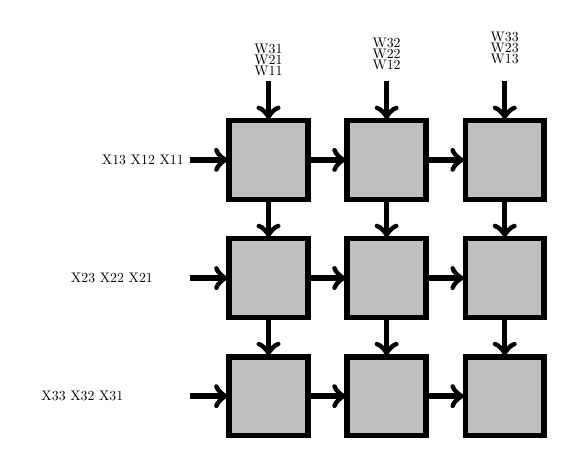
\begin{tikzpicture}[line width=2pt,scale=0.5,transform shape]
\node (M11)[rectangle,minimum width=1cm,minimum size=2cm,draw,fill=lightgray] at (0,0) {};
\node (M21)[rectangle,minimum width=1cm,minimum size=2cm,draw,fill=lightgray] at (3,0) {};
\node (M31)[rectangle,minimum width=1cm,minimum size=2cm,draw,fill=lightgray] at (6,0) {};

\node (M12)[rectangle,minimum width=1cm,minimum size=2cm,draw,fill=lightgray] at (0,-3) {};
\node (M22)[rectangle,minimum width=1cm,minimum size=2cm,draw,fill=lightgray] at (3,-3) {};
\node (M32)[rectangle,minimum width=1cm,minimum size=2cm,draw,fill=lightgray] at (6,-3) {};

\node (M13)[rectangle,minimum width=1cm,minimum size=2cm,draw,fill=lightgray] at (0,-6) {};
\node (M23)[rectangle,minimum width=1cm,minimum size=2cm,draw,fill=lightgray] at (3,-6) {};
\node (M33)[rectangle,minimum width=1cm,minimum size=2cm,draw,fill=lightgray] at (6,-6) {};


\draw[<-] (M11)-- ++(0,2cm) node(W11)[above]{W11};
\node[above] (W21) at (W11) {W21};
\node[above] (W31) at (W21) {W31};
\draw[<-] (M21)-- ++(0,2cm) node(W12)[above]{};
\node[above] (W22) at (W12) {W12};
\node[above] (W32) at (W22) {W22};
\node[above] (W42) at (W32) {W32};
\draw[<-] (M31)-- ++(0,2cm) node(W13)[above]{};
\node[above] (W23) at (W13) {};
\node[above] (W33) at (W23) {W13};
\node[above] (W43) at (W33) {W23};
\node[above] (W53) at (W43) {W33};

\draw[<-] (M11) -- ++(-2cm,0) node[left]{X13 X12 X11};
\draw[->] (M11) -- (M21);
\draw[->] (M21) -- (M31);

\draw[->] (M11) -- (M12);
\draw[->] (M21) -- (M22);
\draw[->] (M31) -- (M32);


\draw[<-] (M12) -- ++(-2cm,0) node[left,minimum width=1.5cm](X2){};
\node[left] at (X2) {X23 X22 X21};
\draw[->] (M12) -- (M22);
\draw[->] (M22) -- (M32);

\draw[->] (M12) -- (M13);
\draw[->] (M22) -- (M23);
\draw[->] (M32) -- (M33);

\draw[<-] (M13) -- ++(-2cm,0) node[left,minimum width=3cm](X3){};
\node[left] at (X3) {X33 X32 X31};
\draw[->] (M13) -- (M23);
\draw[->] (M23) -- (M33);

\node at (-6,0){};
\end{tikzpicture}
}
\hfil
\subfloat[First Step]{
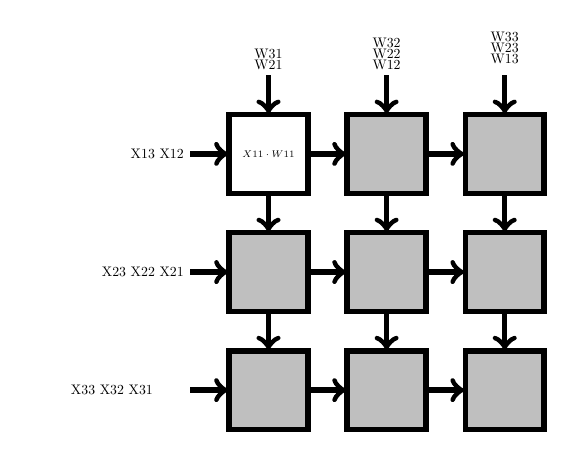
\begin{tikzpicture}[line width=2pt,scale=0.5,transform shape]
\node (M11)[rectangle,minimum size=2cm,draw] at (0,0) {};
\node (M21)[rectangle,minimum size=2cm,draw,fill=lightgray] at (3,0) {};
\node (M31)[rectangle,minimum size=2cm,draw,fill=lightgray] at (6,0) {};

\node (M12)[rectangle,minimum size=2cm,draw,fill=lightgray] at (0,-3) {};
\node (M22)[rectangle,minimum size=2cm,draw,fill=lightgray] at (3,-3) {};
\node (M32)[rectangle,minimum size=2cm,draw,fill=lightgray] at (6,-3) {};

\node (M13)[rectangle,minimum size=2cm,draw,fill=lightgray] at (0,-6) {};
\node (M23)[rectangle,minimum size=2cm,draw,fill=lightgray] at (3,-6) {};
\node (M33)[rectangle,minimum size=2cm,draw,fill=lightgray] at (6,-6) {};


\draw[<-] (M11)-- ++(0,2cm) node(W11)[above]{W21};
\node[above] (W21) at (W11) {W31};
\draw[<-] (M21)-- ++(0,2cm) node(W12)[above]{W12};
\node[above] (W22) at (W12) {W22};
\node[above] (W32) at (W22) {W32};
\draw[<-] (M31)-- ++(0,2cm) node(W13)[above]{};
\node[above] (W23) at (W13) {W13};
\node[above] (W33) at (W23) {W23};
\node[above] (W43) at (W33) {W33};

\draw[<-] (M11) -- ++(-2cm,0) node[left]{X13 X12};
\draw[->] (M11) -- (M21);
\draw[->] (M21) -- (M31);

\draw[->] (M11) -- (M12);
\draw[->] (M21) -- (M22);
\draw[->] (M31) -- (M32);


\draw[<-] (M12) -- ++(-2cm,0) node[left](X2){X23 X22 X21};
\draw[->] (M12) -- (M22);
\draw[->] (M22) -- (M32);

\draw[->] (M12) -- (M13);
\draw[->] (M22) -- (M23);
\draw[->] (M32) -- (M33);

\draw[<-] (M13) -- ++(-2cm,0) node[left,minimum width=1.5cm](X3){};
\node[left] at (X3) {X33 X32 X31};
\draw[->] (M13) -- (M23);
\draw[->] (M23) -- (M33);

\node at (0,0) {\scriptsize $X11\cdot W11$};
\node at (-6,0){};
\end{tikzpicture}
}

\subfloat[Second Step]{
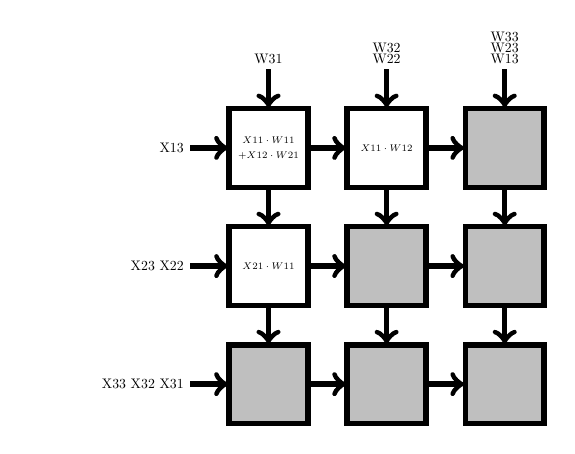
\begin{tikzpicture}[line width=2pt,scale=0.5,transform shape]
\node (M11)[rectangle,minimum size=2cm,draw] at (0,0){};
\node (M21)[rectangle,minimum size=2cm,draw] at (3,0) {};
\node (M31)[rectangle,minimum size=2cm,draw,fill=lightgray] at (6,0) {};

\node (M12)[rectangle,minimum size=2cm,draw] at (0,-3) {};
\node (M22)[rectangle,minimum size=2cm,draw,fill=lightgray] at (3,-3) {};
\node (M32)[rectangle,minimum size=2cm,draw,fill=lightgray] at (6,-3) {};

\node (M13)[rectangle,minimum size=2cm,draw,fill=lightgray] at (0,-6) {};
\node (M23)[rectangle,minimum size=2cm,draw,fill=lightgray] at (3,-6) {};
\node (M33)[rectangle,minimum size=2cm,draw,fill=lightgray] at (6,-6) {};


\draw[<-] (M11)-- ++(0,2cm) node(W11)[above]{W31};
\draw[<-] (M21)-- ++(0,2cm) node(W12)[above]{W22};
\node[above] (W22) at (W12) {W32};
\draw[<-] (M31)-- ++(0,2cm) node(W13)[above]{W13};
\node[above] (W23) at (W13) {W23};
\node[above] (W33) at (W23) {W33};

\draw[<-] (M11) -- ++(-2cm,0) node[left]{X13};
\draw[->] (M11) -- (M21);
\draw[->] (M21) -- (M31);

\draw[->] (M11) -- (M12);
\draw[->] (M21) -- (M22);
\draw[->] (M31) -- (M32);


\draw[<-] (M12) -- ++(-2cm,0) node[left](X2){X23 X22};
\draw[->] (M12) -- (M22);
\draw[->] (M22) -- (M32);

\draw[->] (M12) -- (M13);
\draw[->] (M22) -- (M23);
\draw[->] (M32) -- (M33);

\draw[<-] (M13) -- ++(-2cm,0) node[left](X3){X33 X32 X31};
\draw[->] (M13) -- (M23);
\draw[->] (M23) -- (M33);

\node at (0,0.2){\scriptsize $X11\cdot W11$};
\node at (0,-0.2){\scriptsize $+X12\cdot W21$};
\node at (3,0){\scriptsize $X11\cdot W12$};
\node at (0,-3){\scriptsize $X21\cdot W11$};
\node at (-6,0){};
\end{tikzpicture}
}
\hfil
\hfil
\subfloat[Final Step]{
\begin{tikzpicture}[line width=2pt,scale=0.5,transform shape]
\node (M11)[rectangle,minimum size=2cm,draw] at (0,0) {};
\node (M21)[rectangle,minimum size=2cm,draw] at (3,0) {};
\node (M31)[rectangle,minimum size=2cm,draw] at (6,0) {};

\node (M12)[rectangle,minimum size=2cm,draw] at (0,-3) {};
\node (M22)[rectangle,minimum size=2cm,draw] at (3,-3) {};
\node (M32)[rectangle,minimum size=2cm,draw] at (6,-3) {};

\node (M13)[rectangle,minimum size=2cm,draw] at (0,-6) {};
\node (M23)[rectangle,minimum size=2cm,draw] at (3,-6) {};
\node (M33)[rectangle,minimum size=2cm,draw] at (6,-6) {};


\draw[<-] (M11)-- ++(0,2cm); 
\node[above] (W21) at (W11) {W31};
\draw[<-] (M21)-- ++(0,2cm);
\node[above] (W22) at (W12) {W22};
\node[above] (W32) at (W22) {W32};
\draw[<-] (M31)-- ++(0,2cm);
\node[above] (W23) at (W13) {W13};
\node[above] (W33) at (W23) {W23};
\node[above] (W43) at (W33) {W33};

\draw[<-] (M11) -- ++(-2cm,0);
\draw[->] (M11) -- (M21);
\draw[->] (M21) -- (M31);

\draw[->] (M11) -- (M12);
\draw[->] (M21) -- (M22);
\draw[->] (M31) -- (M32);


\draw[<-] (M12) -- ++(-2cm,0);
\draw[->] (M12) -- (M22);
\draw[->] (M22) -- (M32);

\draw[->] (M12) -- (M13);
\draw[->] (M22) -- (M23);
\draw[->] (M32) -- (M33);

\draw[<-] (M13) -- ++(-2cm,0);
\draw[->] (M13) -- (M23);
\draw[->] (M23) -- (M33);

\node at (0,0.4)  {\scriptsize $ X11\cdot W11$};
\node at (0,0)    {\scriptsize $+X12\cdot W21$};
\node at (0,-0.4) {\scriptsize $+X13\cdot W31$};

\node at (3,0.4)  {\scriptsize $ X11\cdot W12$};
\node at (3,0)    {\scriptsize $+X12\cdot W22$};
\node at (3,-0.4) {\scriptsize $+X13\cdot W32$};

\node at (6,0.4)  {\scriptsize $ X11\cdot W13$};
\node at (6,0)    {\scriptsize $+X12\cdot W23$};
\node at (6,-0.4) {\scriptsize $+X13\cdot W33$};

\node at (0,-2.6) {\scriptsize $ X21\cdot W11$};
\node at (0,-3)   {\scriptsize $+X22\cdot W21$};
\node at (0,-3.4) {\scriptsize $+X23\cdot W31$};

\node at (3,-2.6) {\scriptsize $ X21\cdot W12$};
\node at (3,-3)   {\scriptsize $+X22\cdot W22$};
\node at (3,-3.4) {\scriptsize $+X23\cdot W32$};

\node at (6,-2.6) {\scriptsize $ X21\cdot W13$};
\node at (6,-3)   {\scriptsize $+X22\cdot W23$};
\node at (6,-3.4) {\scriptsize $+X23\cdot W33$};

\node at (0,-5.6) {\scriptsize $ X31\cdot W11$};
\node at (0,-6)   {\scriptsize $+X32\cdot W21$};
\node at (0,-6.4) {\scriptsize $+X33\cdot W31$};

\node at (3,-5.6) {\scriptsize $ X31\cdot W12$};
\node at (3,-6)   {\scriptsize $+X32\cdot W22$};
\node at (3,-6.4) {\scriptsize $+X33\cdot W32$};

\node at (6,-5.6) {\scriptsize $ X31\cdot W13$};
\node at (6,-6)   {\scriptsize $+X32\cdot W23$};
\node at (6,-6.4) {\scriptsize $+X33\cdot W33$};
\node at (-6,0){};
\end{tikzpicture}
}
\end{figure}

\end{document}
